\documentclass[oneside,11pt]{aghdpl}

% \documentclass[oneside,11pt]{aghdpl}
% \documentclass[en,11pt]{aghdpl}  % praca w języku angielskim

% Lista wszystkich języków stanowiących języki pozycji bibliograficznych użytych w pracy.
% (Zgodnie z zasadami tworzenia bibliografii każda pozycja powinna zostać utworzona zgodnie z zasadami języka, w którym dana publikacja została napisana.)
\usepackage[english,polish]{babel}

% Użyj polskiego łamania wyrazów (zamiast domyślnego angielskiego).
\usepackage{polski}

\usepackage[utf8]{inputenc}

% dodatkowe pakiety

\usepackage{mathtools}
\usepackage{amsfonts}
\usepackage{listings}
\usepackage{xcolor}
\usepackage{amsmath}
\usepackage{amsthm}
\usepackage{fancyvrb}

\makeatletter
\newcommand{\setappendix}{Dodatek~\thechapter.~}
\newcommand{\setchapter}{\thechapter~}
\titleformat{\chapter}{\bfseries\LARGE}{%
  \ifnum\pdfstrcmp{\@currenvir}{appendices}=0
    \setappendix
  \else
    \setchapter
  \fi}{0em}{}
\makeatother
\usepackage[titletoc]{appendix}


% --- < bibliografia > ---

\usepackage[
    style=numeric,
    sorting=none,
    %
    % Zastosuj styl wpisu bibliograficznego właściwy językowi publikacji.
    language=autobib,
    autolang=other,
    % Zapisuj datę dostępu do strony WWW w formacie RRRR-MM-DD.
    urldate=iso8601,
    % Nie dodawaj numerów stron, na których występuje cytowanie.
    backref=false,
    % Podawaj ISBN.
    isbn=true,
    % Nie podawaj URL-i, o ile nie jest to konieczne.
    url=false,
    %
    % Ustawienia związane z polskimi normami dla bibliografii.
    maxbibnames=3,
    % Jeżeli używamy BibTeXa:
    backend=bibtex
]{biblatex}

\usepackage{csquotes}
% Ponieważ `csquotes` nie posiada polskiego stylu, można skorzystać z mocno zbliżonego stylu chorwackiego.
\DeclareQuoteAlias{croatian}{polish}

\addbibresource{bibliografia.bib}

% Nie wyświetlaj wybranych pól.
%\AtEveryBibitem{\clearfield{note}}


% ------------------------
% --- < listingi > ---

% Użyj czcionki kroju Courier.
\usepackage{courier}

\usepackage{listings}
\lstloadlanguages{TeX}

\lstset{
    literate={ą}{{\k{a}}}1
    {ć}{{\'c}}1
    {ę}{{\k{e}}}1
    {ó}{{\'o}}1
    {ń}{{\'n}}1
    {ł}{{\l{}}}1
    {ś}{{\'s}}1
    {ź}{{\'z}}1
    {ż}{{\.z}}1
    {Ą}{{\k{A}}}1
    {Ć}{{\'C}}1
    {Ę}{{\k{E}}}1
    {Ó}{{\'O}}1
    {Ń}{{\'N}}1
    {Ł}{{\L{}}}1
    {Ś}{{\'S}}1
    {Ź}{{\'Z}}1
    {Ż}{{\.Z}}1,
    basicstyle=\footnotesize\ttfamily,
}

% ------------------------

\AtBeginDocument{
    \renewcommand{\tablename}{Tabela}
    \renewcommand{\figurename}{Rys.}
}

% ------------------------
% --- < tabele > ---

\usepackage{array}
\usepackage{tabularx}
\usepackage{multirow}
\usepackage{booktabs}
\usepackage{makecell}
\usepackage[flushleft]{threeparttable}

% defines the X column to use m (\parbox[c]) instead of p (`parbox[t]`)
\newcolumntype{C}[1]{>{\hsize=#1\hsize\centering\arraybackslash}X}

\DefineBibliographyStrings{english}{%
  urlseen = {dostęp dnia},
}

%---------------------------------------------------------------------------

\author{Kacper Żuk}
\shortauthor{K. Żuk}

\titlePL{Opracowanie biblioteki programistycznej do bezpiecznego uwierzytelniania urządzeń AVR.}
\titleEN{Development of libraries for authentication of AVR devices.}

\shorttitlePL{Opracowanie biblioteki programistycznej do bezpiecznego uwierzytelniania urządzeń AVR.}
\shorttitleEN{Development of libraries for authentication of AVR devices.}

\thesistype{Praca dyplomowa inżynierska}

\supervisor{dr inż. Jarosław Bułat}

\degreeprogramme{Teleinformatyka}

\date{2016}

\department{Katedra Telekomunikacji}

%\faculty{Wydział Elektrotechniki, Automatyki,\protect\\[-1mm] Informatyki i Inżynierii Biomedycznej}
\faculty{Wydział Informatyki, Elektroniki i Telekomunikacji}
%\faculty{Faculty of Electrical Engineering, Automatics, Computer Science and Biomedical Engineering}

% FIXME podziekowania?
\acknowledgements{}


\setlength{\cftsecnumwidth}{10mm}

%---------------------------------------------------------------------------
\setcounter{secnumdepth}{4}
\brokenpenalty=10000\relax

%\newcommand*{\thead}[1]{\multicolumn{1}{c}{\bfseries #1}}

\begin{document}

\titlepages

% Ponowne zdefiniowanie stylu `plain`, aby usunąć numer strony z pierwszej strony spisu treści i poszczególnych rozdziałów.
\fancypagestyle{plain}
{
    % Usuń nagłówek i stopkę
    \fancyhf{}
    % Usuń linie.
    \renewcommand{\headrulewidth}{0pt}
    \renewcommand{\footrulewidth}{0pt}
}

\setcounter{tocdepth}{2}
\tableofcontents
\clearpage

\chapter*{Wprowadzenie}
\addcontentsline{toc}{chapter}{Wprowadzenie}
\label{cha:wstep}

\begin{figure}[h]
\centering
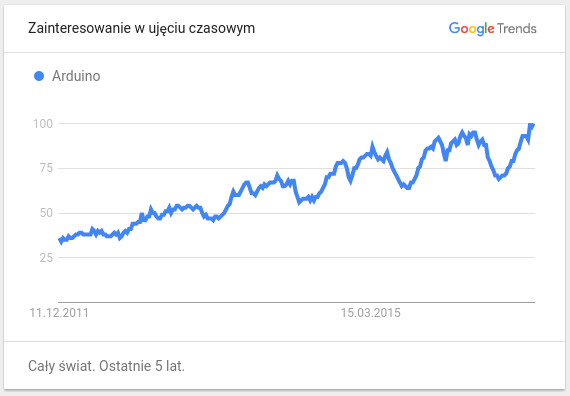
\includegraphics[width=0.7\textwidth]{images/arduino-trends.png}
\caption{Relatywna liczba wyszukiwań frazy ,,Arduino'' w ostatnich pięciu latach. Źródło: Google Trends}
\label{fig:arduinotrends}
\end{figure}

AVR to rodzina mikroprocesorów opracowana i~rozwijana przez firmę Atmel. Oparta o~nią jest między innymi platforma Arduino, która~-- jak~przedstawiono na~rysunku \ref{fig:arduinotrends} -- z~roku na~rok zyskuje popularność. Platforma Arduino zaprojektowana została z~myślą o~projektach tworzonych nie tylko przez inżynierów, lecz także artystów i~projektantów~\cite{BanShi14}. Jest ona też często używana do~prototypowania urządzeń wpisujących się w~koncepcję Internetu Rzeczy \emph{(ang. Internet of Things, IoT)}.

Urządzenia wbudowane podłączone do~Internetu są szczególnie narażone na~ataki. W~2016 roku podatne urządzenia wbudowane zostały wykorzystane do~przeprowadzenia masywnych ataków typu DDoS~\cite{AkaIOT}. Zagrożone są też rozwiązania oparte o~komunikację bezprzewodową jak~Wi-Fi oraz~Bluetooth. Istotne jest więc dostarczenie narzędzi, które~pozwalają nie tylko na~szybkie prototypowanie, ale~także na~zachowanie bezpieczeństwa takich rozwiązań jak~bezprzewodowe tokeny, czujniki, sprzętowe menadżery haseł czy~inteligentne domy.

W~niniejszej pracy przedstawiono protokół bezpiecznej komunikacji oraz~bibliotekę programistyczną zaprojektowane z~myślą o~prostocie integracji. Wybrane zostały zestawy algorytmów, które~zapewniają bezpieczeństwo komunikacji. Ich złożoność została ukryta za~interfejsem programistycznym, który~ogranicza możliwość wprowadzenia błędów zmniejszających bezpieczeństwo. Zaproponowane rozwiązanie zapewnia poufność, autentyczność oraz~integralność przesyłanych danych.

W~rozdziale \ref{cha:metodyUwierzytelniania} przedstawione zostały różne metody uwierzytelniania i~uzasadniony został wybór konkretnych algorytmów. Implementacja została szczegółowo opisana w~rozdziale \ref{cha:implementacja}. Całość została zweryfikowana poprzez~strzorzenie przykładowego oprogramowania oraz~porównanie z~implementacją na~inną platformę, co opisano w~rozdziale \ref{cha:walidacja}. W~podsumowaniu przedstawiono całe rozwiązanie oraz~jego ograniczenia i~słabe strony.

Całość kodu źródłowego dostępna jest na~licencji MIT w~serwisie GitHub\footnote{\url{https://github.com/kacperzuk/seconn}}.

\chapter{Charakterystyka platformy sprzętowej}
\label{cha:hardware}

Mikropocesory Atmel AVR są w większości 8-bitowe i na takich skupia się praca. Rodzina AVR jest szeroka, kilka wybranych modeli przedstawiono w tabeli \ref{tab:avrmodels}. W pracy wykorzystany został model ATmega32u4 z 2,5 kilobajta SRAM~\cite{Atmega32}.

\begin{table}[h]
\centering
\caption{Wybrane modele AVR wraz z ich parametrami}
\begin{tabular}{|l|l|l|l|l|}
    \hline
    \textbf{Nazwa}  &
    \textbf{SRAM\footnote{ang. Static Random Access Memory}}  &
    \textbf{Wymagane napięcie}  &
    \textbf{Taktowanie procesora}  &
    \textbf{Liczba linii I/O} \\
    \hline
    ATtiny4 \cite{Attiny4}& 32 B & 1.8 - 5.5 V & do 12 MHz & 4\\
    \hline
    ATmega32u4 \cite{Atmega32} & 2,5 KB & 2.7 - 5.5 V & do 16 MHz & 26\\
    \hline
    ATxmega384C3 \cite{Atxmega384} & 32 KB & 1.6 - 3.6 V & do 32 MHz & 50\\
    \hline
\end{tabular}
\label{tab:avrmodels}
\end{table}

SRAM jest głównym ograniczeniem w implementacji uwierzytelniania, ponieważ 32 bajty nie są wystaczające do przeprowadzania operacji kryptograficznych, przy których sam klucz zajmuje 16 lub 32 bajty. Należy też pamiętać, że obsługa bezpiecznego połączenia nie może zajmować całości pamięci. Część pamięci należy przeznaczyć na obsługę peryferiów oraz właściwą logikę programu.

Istotnym elementem jest też wielkość domyślnych buforów. \emph{Arduino} w modułach \emph{Serial} oraz \emph{SoftwareSerial} domyślnie używa 16- lub 64-bajtowego (w zależności od ilości dostępnej pamięci) buforu na przychodzące dane\footnote{https://github.com/arduino/Arduino/blob/master/hardware/arduino/avr/cores/arduino/HardwareSerial.h}. Przy wiadomościach dłuższych niż 32 bajty oznacza to, że zbyt długie przetwarzanie jednej wiadomości spowoduje błędne odebranie następnej, jeżeli zostanie ona za szybko wysłana.

Maksymalne taktowanie mikroprocesora zależy od konkretnego modelu (od 12 do 32 MHz) oraz napięcia zasilania. Wykorzystywany w pracy Atmega32u4 zasilany był napięciem 5 V, co przekłada się na taktowanie 16 MHz.

\chapter{Metody uwierzytelniania}
\label{cha:metodyUwierzytelniania}

W~zależności od~potrzeb i~ograniczeń stosuje się różne metody uwierzytelniania podmiotów w~komunikacji. Wyróżnić należy uwierzytelnianie przy pomocy kryptografii asymetrycznej, w~której używana jest para matematycznie związanych ze~sobą kluczy, oraz~uwierzytelnianie przy pomocy kryptografii symetrycznej, w~której używany jest jeden, współdzielony, tajny klucz.

Klucze w~przypadku kryptografii asymetrycznej muszą posiadać konkretne właściwości. W~przypadku algorytmu RSA bezpieczeństwo polega na~trudności w~faktoryzowaniu dużych liczb, co wymaga stosowania kluczy co najmniej 2048 bitowych~\cite{Nist}. Klucze w~przypadku kryptografii symetrycznej nie muszą mieć konkretnych właściwości poza ich nieprzewidywalnością i~zapewniają porównywalne bezpieczeństwo przy krótszych kluczach. Kluczowi RSA o~długości 2048 bitów odpowiada klucz 112 bitowy dla szyfrów symetrycznych.

Ważną różnicą jest też wydajność. Kryptografia asymetryczna jest dużo bardziej złożona obliczeniowo od~symetrycznej~\cite{al2008comparative}. Jest to szczególnie istotne na~ograniczonych sprzętowo systemach wbudowanych. Przewagą kryptografii asymetrycznej jest jednak brak konieczności ustalenia wspólnego klucza przed rozpoczęciem komunikacji, jak~ma to miejsce w~przypadku kryptografii symetrycznej.

Zalecanym rozwiązaniem jest najpierw ustalenie wspólnego, tajnego klucza przy użyciu kryptografii asymetrycznej, a~następnie użycie tego klucza do~kryptografii symetrycznej~\cite{al2008comparative}.

\section{Kryptografia asymetryczna}
\label{sec:kryptoAsym}

Przy wyborze algorytmu używanego do~ustalania klucza dla potrzeb pracy istotne były:

\begin{itemize}
\item jakość implementacji algorytmów dostępnych na mikroprocesory AVR,
\item złożoność obliczeniowa,
\item długość klucza wymagana do zapewnienia bezpieczeństwa na co najmniej 5 lat.
\end{itemize}

Biblioteka \emph{AVR-Crypto-Lib} dostarcza implementację algorytmów RSA oraz~DSA\footnote{\url{https://trac.cryptolib.org/avr-crypto-lib/browser}}. Biblioteka \emph{Emsign} dostarcza implementację RSA, lecz tylko z~64 bitowym kluczem\footnote{\url{http://www.emsign.nl/}}, co nie jest wystarczające dla zapewnienia bezpieczeństwa. Komercyjna biblioteka \emph{LightCrypt-AVR8-ECC} oraz~biblioteka \emph{micro-ecc} dostarczają implementację kryptografii opartej o~krzywe eliptyczne\footnote{\url{http://industrial.crypto.cmmsigma.eu/lightcrypt_avr8/lc_avr8_ecc.pl.html}}. Brak jest na~rynku implementacji innych algorytmów klucza publicznego. Dostępność implementacji ogranicza wybór algorytmu do~RSA, DSA oraz~krzywych eliptycznych.

Następnym kryterium jest złożoność obliczeniowa. W~analizie przeprowadzonej przez pracowników \emph{Sun Microsystems Laboratories} wykazano, że~na mikroprocesorach AVR algorytmy oparte o~krzywe eliptyczne są o~rząd wielkości szybsze od~algorytmu RSA~\cite{Gura2004}.

Krzywe eliptyczne wymagają najkrótszych kluczy. Rekomendacje NIST~\cite{Nist} (National Institute of Standards and Technology) podają, że~256-bitowy klucz ECC (ang. \emph{Elliptic Curve Cryptography}) zapewnia bezpieczeństwo porównywalne do~3072-bitowego klucza RSA lub~DSA i~że taki klucz wystarczy do~2030 roku.

W~związku z~przewagą krzywych eliptycznych przy zadanych założeniach do~ustalenia wspólnego klucza wybrano algorytm ECDH (ang. \emph{Elliptic Curve Diffie--Hellman}). Wadą tego rozwiązania jest niezmienność klucza ustalanego tą metodą. Powoduje to brak utajnienia przekazywania (ang. \emph{forward secrecy}).

\section{Kryptografia symetryczna}
\label{sec:kryptoSym}

Przy wyborze algorytmu dla potrzeb pracy istotne były:

\begin{itemize}
\item jakość implementacji dostępnych na mikroprocesory AVR,
\item możliwość szyfrowania i uwierzytelniania danych.
\end{itemize}

Powszechnie dostępne są jedynie implementacje samych blokowych algorytmów szyfrowania takich jak~AES oraz~DES lub~funkcji skrótu takich jak~SHA-256. By~uzyskać uwierzytelnianie wiadomości o~zmiennej długości należy algorytmy blokowe zastosować w odpowiedni sposób. Przykładem jest tryb CBC-MAC {\itshape (ang. Cipher Block Chaining - Message Authentication Code)}. Pozwala on na~wygenerowanie kodu uwierzytelniającego daną wiadomość, poprzez~zaszyfrowanie jej w~trybie CBC i~użycie ostatniego bloku szyfrogramu jako kodu.

\begin{figure}[ht]
\centering
\includegraphics[width=\textwidth]{images/cbc.png}
\caption{Schemat działania trybu CBC.}
\label{fig:cbc}
\end{figure}

W~trybie CBC z~każdego 16 bajtowego bloku danych oraz~szyfrogramu bloku poprzedzającego liczona jest suma modulo 2, co przedstawiono na~rysunku \ref{fig:cbc}. Wektor inicjalizacyjny jest stosowany, by~dwie wiadomości o~identycznym pierwszym 16 bajtowym bloku po~zaszyfrowaniu nie miały identycznego pierwszego bloku szyfrogramu. By~wektor inicjalizacyjny poprawnie pełnił taką rolę, musi być losowy i~przesyłany do~odbiorcy. Nie musi być on tajny. W~przypadku trybu CBC-MAC używany jest jedynie ostatni blok szyfrogramu, a~więc wektor inicjalizacyjny nie jest potrzebny. Zwyczajowo korzysta się więc z~wektora inicjalizacyjnego wypełnionego zerami.

\FloatBarrier

Tryb CBC-MAC -- przy nieprawidłowej implementacji -- może wprowadzić podatności:

\begin{itemize}
    \item użycie zmiennego wektora inicjalizacyjnego i~przesyłanie go wraz z~uwierzytelnianą wiadomością pozwala na~dowolną modyfikację pierwszego bloku (16 bajtów) wiadomości bez zmiany kodu uwierzytelniającego,
    \item użycie tego samego klucza do~szyfrowania w~trybie CBC oraz~uwierzytelniania w~trybie CBC-MAC pozwala na~obliczenie użytego klucza bez jego wcześniejszej znajomości,
    \item atakujący znający dwie wiadomości $ m $ oraz~$ m' $ oraz~ich kody uwierzytelniające może policzyć klucz uwierzytelniający wiadomości będącej specyficznym połączeniem wiadomości $ m $ oraz~$ m' $.
\end{itemize}

Wszystkim tym podatnościom da się zapobiec poprzez~użycie niezmiennego wektora inicjalizacyjnego oraz~zaszyfrowanie ostatniego bloku innym kluczem (tryb ECBC-MAC, {\itshape ang. Encrypt-last-block CBC-MAC}).

Alternatywą jest także zastosowanie HMAC {\itshape (ang. keyed-hash message authentication code)}. Kodem uwierzytelniającym jest wtedy wynik funkcji skrótu policzony z~połączenia współdzielonego klucza oraz~uwierzytelnianej wiadomości \cite{krawczyk1997hmac}.

W~pracy do~uwierzytelniania wybrano AES w~trybie ECBC-MAC. Zaletą tego rozwiązania jest możliwość użycia tej samej implementacji trybu CBC zarówno do~szyfrowania jak~i~jako element trybu ECBC-MAC.

W~implementacji szyfrowania w~trybie CBC należało rozwiązać problemy wymienione poniżej.

\begin{enumerate}
    \item Użycie przewidywalnych wektorów inicjalizacyjnych pozwala atakującemu na~zgadywanie treści wiadomości, a~następnie -- poprzez~odpowiednie spreparowanie nowej wiadomości -- weryfikację, czy~wiadomość się zgadza. Wektory inicjalizacyjne muszą być nieprzewidywalne.
    \item CBC operuje na~blokach danych, a~więc dla wiadomości o~długości niebędącej wielokrotnością długości bloku wymagane jest dopełnienie. Oznacza to że~do~szyfrowanej wiadomości należy dołączać jej długość lub~użyć dopełnienia, które~jest jednoznaczne.
\end{enumerate}

Szyfrowanie z~uwierzytelnianiem jest połączone wedle zasady {\itshape Encrypt-then-MAC}. Oznacza to że~wiadomość najpierw jest szyfrowana, a~następnie uwierzytelniany jest szyfrogram, a~nie bezpośrednio wiadomość. Jest to rozwiązanie zapewniające najwyższe bezpieczeństwo, zapobiegające między innymi atakom typu \emph{padding oracle}~\cite{black2011authenticated}. Całość procesu została przedstawiona na~rysunku \ref{fig:etm}.

\begin{figure}[ht]
\centering
\includegraphics[width=0.6\textwidth]{images/etm.png}
\caption{Proces szyfrowania i uwierzytelniania danych}
\label{fig:etm}
\end{figure}

\chapter{Implementacja protokołu komunikacji}
\label{cha:implementacja}

Protokół komunikacji między dwoma węzłami zaprojektowano i zaimplementowano z następującymi założeniami:

\begin{itemize}
\item pełna funkcjonalność przy jak najmniejszych wymaganiach sprzętowych, w szczególności przy dostępnej małej ilości pamięci operacyjnej,
\item częściowa niezależność od warstwy sieciowej,
\item zapewnienie uwierzytelniania i szyfrowania wiadomości.
\end{itemize}

\section{Charakterystyka platformy sprzętowej}
\label{cha:hardware}

Mikropocesory Atmel AVR są w większości 8-bitowe i na takich skupia się praca. Rodzina AVR jest szeroka, kilka wybranych modeli przedstawiono w tabeli \ref{tab:avrmodels}. W pracy wykorzystany został model ATmega32u4 z 2,5 kilobajta SRAM~\cite{Atmega32}.

\begin{table}[h]
\centering
\caption{Wybrane modele AVR wraz z ich parametrami}
\begin{tabular}{|l|l|l|l|l|}
    \hline
    \textbf{Nazwa}  &
    \textbf{SRAM\footnote{ang. Static Random Access Memory}}  &
    \textbf{Wymagane napięcie}  &
    \textbf{Taktowanie procesora}  &
    \textbf{Liczba linii I/O} \\
    \hline
    ATtiny4 \cite{Attiny4}& 32 B & 1.8 - 5.5 V & do 12 MHz & 4\\
    \hline
    ATmega32u4 \cite{Atmega32} & 2,5 KB & 2.7 - 5.5 V & do 16 MHz & 26\\
    \hline
    ATxmega384C3 \cite{Atxmega384} & 32 KB & 1.6 - 3.6 V & do 32 MHz & 50\\
    \hline
\end{tabular}
\label{tab:avrmodels}
\end{table}

SRAM jest głównym ograniczeniem w implementacji uwierzytelniania, ponieważ 32 bajty nie są wystaczające do przeprowadzania operacji kryptograficznych, przy których sam klucz zajmuje 16 lub 32 bajty. Należy też pamiętać, że obsługa bezpiecznego połączenia nie może zajmować całości pamięci. Część pamięci należy przeznaczyć na obsługę peryferiów oraz właściwą logikę programu.

Istotnym elementem jest też wielkość domyślnych buforów. \emph{Arduino} w modułach \emph{Serial} oraz \emph{SoftwareSerial} domyślnie używa 16- lub 64-bajtowego (w zależności od ilości dostępnej pamięci) buforu na przychodzące dane\footnote{https://github.com/arduino/Arduino/blob/master/hardware/arduino/avr/cores/arduino/HardwareSerial.h}. Przy wiadomościach dłuższych niż 32 bajty oznacza to, że zbyt długie przetwarzanie jednej wiadomości spowoduje błędne odebranie następnej, jeżeli zostanie ona za szybko wysłana.

\section{Podstawowe struktury protokołu}
\label{sec:proto}

\begin{figure}[h]
\centering
\includegraphics[width=\textwidth]{images/wiadomosc.png}
\caption{Budowa wiadomości w protokole komunikacji.}
\label{fig:message-def}
\end{figure}

\begin{table}[t]
\centering
\caption{Typy wiadomości wraz z ich charakterystyką}
\begin{tabular}{|p{2.3cm}|p{1.4cm}|l|p{2.9cm}|p{3.1cm}|}
    \hline
    \textbf{Typ \mbox{wiadomości}}  &
    \textbf{Wartość pola typ}  &
    \textbf{Długość bloku danych}  &
    \textbf{Blok danych jest zaszyfrowany}  &
    \textbf{Blok danych jest uwierzytelniony}\\
    \hline
    HelloRequest & 0x00 & 64 bajty & nie & nie\\
    \hline
    HelloResponse & 0x01 & 96 bajtów & tak & tak\\
    \hline
    EncryptedData & 0x02 & zmienna, minimum 32 bajty & tak & tak\\
    \hline
\end{tabular}
\label{tab:recordtypes}
\end{table}

Podstawową jednostką protokołu są wiadomości zbudowane według schematu zaprezentowanego na Rys. \ref{fig:message-def}. Zdefiniowane typy wiadomości są przedstawione w tabeli \ref{tab:recordtypes}. Budowę przykładowych wiadomości przedstawiono na rysunkach \ref{fig:hellorequestsample}, \ref{fig:helloresponsesample} oraz \ref{fig:encrypteddatasample} w dodatku \ref{app:samplerecords}.

Odbiorca powinien zweryfikować:

\begin{itemize}
\item zgodność wersji protokołu -- wymagane bajty 0x00 oraz 0x01,
\item prawidłowość bajtu określającego typ -- wymagana wartość 0x00, 0x01 lub 0x02,
\item zgodność zadeklarowanej długości bloku danych z typem,
\item w przypadku typów HelloResponse oraz EncryptedData -- prawidłowość kodu uwierzytelniającego.
\end{itemize}

W przypadku niezgodności któregokolwiek elementu wiadomość powinna zostać zignorowana.

Narzut pamięci operacyjnej implementacji protokołu wynosi około 2 KB. Narzut na rozmiar programu to 14.6 KB.

\section{Nawiązywanie połączenia}

\begin{figure}[h]
\centering
\begin{BVerbatim}
Nawiązujący połączenie              Odbierający połączenie
        |             HelloRequest              |
        |      zawiera KPN (klucz publiczny     |
        |       nawiązującego połączenie)       |
   1.   | +---------------------------------->> |
        |                                       |
        |             HelloRequest              |
        |      zawiera KPO (klucz publiczny     |
        |       odbierającego połączenie)       |
   2.   | <<----------------------------------+ |
        |                                       |
        |             HelloResponse             |
        |      zawiera uwierzytelniony KPN      |
   3.   | +---------------------------------->> |
        |                                       |
        |             HelloResponse             |
        |      zawiera uwierzytelniony KPO      |
   4.   | <<----------------------------------+ |
\end{BVerbatim}
\caption{Kolejność wymiany wiadomości w procesie nawiązywania połączenia}
\label{fig:handshake}
\end{figure}

Kolejność przesyłania wiadomości w celu nawiązania połączenia przedstawiona została na rysunku~\ref{fig:handshake}. HelloRequest zawiera klucz publiczny węzła, który go wysyła. Węzeł, który odbiera HelloRequest, używa swojego klucza publicznego oraz klucza publicznego z odebranej wiadomości do ustalenia sekretnego klucza. Nawiązującym połączenie może być dowolny węzeł.

Po ustaleniu wspólnego klucza węzły mogą wysłać HelloResponse, który zawiera zaszyfrowany i uwierzytelniony klucz publiczny pochodzący z wysyłającego węzła. Jeżeli węzeł odbierający wiadomość skutecznie potwierdzi, że jest ona prawidłowo uwierzytelniona, a zdeszyfrowany klucz publiczny pokrywa się z kluczem przesłanym wcześniej w HelloRequest, połączenie uznawane jest za nawiązane. Jeżeli przed odebraniem HelloResponse odebrany był więcej niż jeden HelloRequest, brana pod uwagę jest wiadomość odebrana jako ostatnia. Po nawiązaniu połączenia wymieniane mogą być tylko wiadomości typu EncryptedData.

Istotne jest, że protokół nie zapewnia autentyczności danego klucza publicznego. Powinno to zostać zweryfikowane niezależnie, na przykład poprzez wyświetlenie skrótu klucza użytkownikowi i poproszenie go o potwierdzenie, że na obu urządzeniach uczestniczących w komunikacji jest wyświetlony taki sam klucz.

Protokół zakłada też, że przesyłanie danych jest niezawodne, połączeniowe oraz zachowana jest ich kolejność. Nie są więc zaimplementowane retransmisje ani wykrywanie, czy drugi węzeł rzeczywiście nasłuchuje na przychodzące dane.

\section{Generowanie współdzielonego klucza}
\label{sec:sharedkey}

Każdy z węzłów po odebraniu HelloRequest używa odebranego klucza publicznego oraz swojego klucza publicznego do ustalenia wspólnego sekretu przy użyciu algorytmu ECDH \emph{(ang. Elliptic curve Diffie--Hellman)} oraz proponowanej przez NIST krzywej eliptycznej P-256~\cite{kerry2013digital} (w RFC 5480 nazwaną krzywą secp256r1~\cite{turner2009elliptic}).

Z sekretu będącego wynikiem algorytmu ECDH liczony jest skrót przy użyciu algorytmu SHA-256. Następnie jest on dzielony na dwie części po 128-bitów. Pierwsza część staje się współdzielonym kluczem używanym do szyfrowania, druga część staje się współdzielonym kluczem używanym do uwierzytelniania.

Implementacja algorytmu ECDH z krzywą eliptyczną P-256 pochodzi z biblioteki \emph{micro-ecc}. Jest to jedyna darmowa biblioteka implementująca ECDH. Wygenerowanie wspólnego sekretu na mikroprocesorze ATmega32u4 trwa do 4350 ms, nie uwzględniając generowania liczb losowych, używanych przez bibliotekę \emph{micro-ecc} do zapobiegania atakom typu \emph{side-channel}. Przy uwzględnieniu generowania liczb losowych metodą opisaną w Dodatku \ref{app:randgen} czas ten rośnie do 4500ms.

\section{Szyfrowanie i deszyfrowanie danych}
\label{sec:encrypt}

Szyfrowanie bloku danych w wiadomości odbywa się za pomocą szyfru blokowego AES ze 128-bitowym kluczem używanym w trybie CBC. Wektor inicjalizacyjny jest losowy i dołączany do danych przesyłanej wiadomości przed szyfrogramem. Tekst jawny jest dopełniany do pełnego bloku według algorytmu zdefiniowanego w PKCS\#7~\cite{kaliski1998pkcs}.

\begin{figure}[h]
\centering
\includegraphics[width=\textwidth]{images/cbc.png}
\caption{Schemat działania trybu CBC.}
\label{fig:cbc}
\end{figure}

W tym trybie z każdego 16 bajtowego blok danych oraz szyfrogramu bloku poprzedzającego liczona jest suma modulo 2, co przedstawiono na rysunku \ref{fig:cbc}. Wektor inicjalizacyjny jest stosowany, by dwie wiadomości o identycznym pierwszym 16 bajtowym bloku po zaszyfrowaniu nie miały identycznego pierwszego bloku szyfrogramu. By wektor inicjalizacyjny poprawnie pełnił taką rolę, musi być losowy i przesyłany do odbiorcy. Nie musi być on tajny.

Stworzona biblioteka nie posiada własnego źródła liczb losowych, musi zostać ono dostarczone w ramach integracji. Przykładowa metoda generowania liczb losowych na platformie Arduino została opisana w Dodatku \ref{app:randgen}.

Właściwe kroki potrzebne do zaszyfrowania danych wypisano poniżej.

\begin{enumerate}
\item Dopełnienie tekstu jawnego do pełnego bloku:
\begin{itemize}
\item jeżeli długość tekstu jawnego jest wielokrotnością długości bloku, do tekstu jawnego doklejone musi być 16 bajtów o wartości 16,
\item w przeciwnym wypadku, gdy wymagane jest dopełnienie $ N $ bajtów, do tekstu jawnego doklejone musi być $ N $ bajtów o wartości $ N $.
\end{itemize}
\item Zaszyfrowanie dopełnionego tekstu jawnego w trybie CBC z losowym wektorem inicjalizacyjnym.
\item Doklejenie wektora inicjalizacyjnego przed szyfrogramem.
\end{enumerate}

Przykłady dopełniania danych o różnych długościach przedstawiono w tabeli~\ref{tab:padding}.

\begin{table}[th]
\centering
\caption{Dopełnanie danych do pełnego bloku. Dopełnienie zaznaczone zostało kolorem niebieskiem i pogrubieniem.}
{\footnotesize Dane ,,Witaj swiecie'' (13 bajtów) zostają dopełnione 3 bajtami o wartości 3 (0x03):}

\texttt{0x57 0x69 0x74 0x61\\
0x6a 0x20 0x73 0x77\\
0x69 0x65 0x63 0x69\\
0x65 {\color[rgb]{0,0,1}\bfseries 0x03 0x03 0x03}}

{\footnotesize Dane ,,Witaj swiecie !!'' (16 bajtów) zostają dopełnione 16 bajtami o wartości 16 (0x10):}

\texttt{0x57 0x69 0x74 0x61\\
0x6a 0x20 0x73 0x77\\
0x69 0x65 0x63 0x69\\
0x65 0x20 0x21 0x21\\
{\color[rgb]{0,0,1}\bfseries
0x10 0x10 0x10 0x10\\
0x10 0x10 0x10 0x10\\
0x10 0x10 0x10 0x10\\
0x10 0x10 0x10 0x10\\
}
}

\label{tab:padding}
\end{table}

Kod implementujący szyfrowanie danych przedstawiono w tabeli~\ref{lst:encrypt} w dodatku~\ref{app:codesamples}. Zaszyfrowanie 32 bajtów danych na mikroprocesorze ATmega32u4 trwa do 8 ms bez uwzględnienia czasu potrzebnego do wygenerowania losowego wektora inicjalizacyjnego. Przy generowaniu losowych danych metodą opisaną w Dodatku \ref{app:randgen} czas ten rośnie do 64 ms.

Właściwe kroki potrzebne do odszyfrowania danych wypisano poniżej.

\begin{enumerate}
\item Oddzielenie wektora inicjalizacyjnego od szyfrogramu.
\item Zdeszyfrowanie szyfrogramu w trybie CBC przy wykorzystaniu oddzielonego wektora inicjalizacyjnego.
\item Pobranie wartości ostatniego bajtu zdeszyfrowanego ciągu:
\begin{itemize}
    \item wartość ta nazywana jest dalej $ N $.
\end{itemize}
\item Zweryfikowanie poprawności dopełnienia:
\begin{itemize}
    \item ostatnie $ N $ bajtów musi mieć wartość $ N $,
    \item jeżeli dopełnienie jest nieprawidłowe, cała wiadomość jest ignorowana.
\end{itemize}
\item Usunięcie ostatnich $ N $ bajtów.
\end{enumerate}

Kod implementujący odszyfrowanie danych przedstawiono w tabeli~\ref{lst:decrypt} w dodatku~\ref{app:codesamples}. Zdeszyfrowanie 32 bajtów danych na mikroprocesorze ATmega32u4 trwa do 8 ms.

Implementacja algorytmu AES pochodzi z biblioteki \emph{AVR-Crypto-Lib}. Jest to najlepiej udokumentowana, darmowa biblioteka implementująca algorytm AES. Implementacja trybu CBC oraz algorytmu dopełniania zostały zrealizowane w ramach pracy.

\section{Uwierzytelnienie wiadomości}
\label{sec:auth}

%todo przyklad uwierzytelnienia

Uwierzytelnienie wiadomości odbywa się poprzez dołączenie MAC do bloku danych. Dla danej wiadomości MAC tworzony jest za pomocą szyfru blokowego AES ze 128-bitowym kluczem używanym w trybie ECBC-MAC. Wektor inicjalizacyjny wypełniony jest zerami i nie jest przesyłany. Uwierzytelniany jest kompletny szyfrogram wraz z wektorem inicjalizacyjnym użytym do szyfrowania, a nie tekst jawny. Długość szyfrogramu wraz z wektorem inicjalizacyjnym zawsze będzie wielokrotnością długości bloku, a więc nie jest stosowane dopełnianie.

Tryb ECBC-MAC to tryb CBC-MAC, którego wynik jest dodatkowo szyfrowany innym kluczem niż ten użyty do CBC-MAC. W tej pracy do CBC-MAC użyty jest klucz służący do uwierzytelniania, a wynik CBC-MAC jest szyfrowany używając klucza służącego do szyfrowania.

Właściwe kroki potrzebne do obliczenia kodu uwierzytelniającego opisano poniżej.

\begin{enumerate}
\item Obliczenie ostatniego bloku będącego wynikiem zaszyfrowania szyfrogramu wraz z wektorem inicjalizacyjnym w trybie CBC z wektorem inicjalizacyjnym wypełnionym zerami przy użyciu klucza przeznaczonego do uwierzytelniania.
\item Zaszyfrowanie bloku przy wykorzystaniu AES i klucza przeznaczonego do szyfrowania.
\end{enumerate}

Węzeł wysyłający dokleja kod uwierzytelniający przed szyfrogramem. Węzeł odbierający oddziela otrzymany kod od szyfrogramu, oblicza kod uwierzytelniający dla danego szyfrogramu i porównuje, czy zgadza się on z kodem otrzymanym. Jeżeli kod obliczony różni się od kodu otrzymanego, cała wiadomość jest ignorowana.

Kod implementujący obliczanie MAC przedstawiono w tabeli~\ref{lst:mac} w dodatku~\ref{app:codesamples}. Wygenerowanie kodu uwierzytelniającego dla 32 bajtów danych na mikroprocesorze ATmega32u4 trwa do 8 ms.

Implementacja trybu ECBC-MAC została zrealizowana w ramach pracy.

\section{Złożoność implementacji}
\label{cha:complexity}

\FloatBarrier

Stworzona biblioteka implementująca protokół posiada cztery zależności:

\begin{itemize}
    \item moduł \emph{AES} z biblioteki \emph{AVR-Crypto-Lib},
    \item moduł \emph{gf256mul} wymagany do obliczeń na dużych liczbach z biblioteki \emph{AVR-Crypto-Lib},
    \item moduł \emph{SHA-256} z biblioteki \emph{AVR-Crypto-Lib},
    \item biblioteka \emph{micro-ecc}.
\end{itemize}

Za pomocą programu \emph{ctags} obliczono, że całość biblioteki wraz z zależnościami składa się ze 131 funkcji oraz 13 struktur. Dla kodu stworzonego w ramach pracy -- po odliczeniu zależności -- liczba funkcji to 13 a struktur to 5. Dodatkowe statystyki dotyczące linii kodu zaprezentowano w tabelach \ref{tab:stats} oraz \ref{tab:statssmall}, odpowiednio uwzględniając i pomijając zależności. Statystyki te wygenerowano przy pomocy programu \emph{cloc}.

\begin{table}[h]
\centering
\caption{Statystyki złożoności kodu źródłowego}
\begin{subtable}{\textwidth}
    \centering
\begin{tabular}{|l|l|l|l|l|}
    \hline
    \textbf{Typ pliku}  &
    \textbf{Liczba plików}  &
    \textbf{Liczba linii komentarzy}  &
    \textbf{Liczba linii kodu} \\
    \hline
    Nagłówek C/C++ & 24 & 921 & 2466 \\
    \hline
    C & 13 & 402 & 1772 \\
    \hline
    C++ & 3 & 11 & 303 \\
    \hline
    Asembler & 1 & 49 & 39 \\
    \hline
    \hline
    \textbf{Suma} &
    \textbf{41} &
    \textbf{1383} &
    \textbf{4580} \\
    \hline
\end{tabular}
\caption{Statystyki złożoności kodu źródłowego biblioteki wraz z zależnościami.}
\label{tab:stats}
\end{subtable}

\begin{subtable}{\textwidth}
    \centering
\begin{tabular}{|l|l|l|l|}
    \hline
    \textbf{Typ pliku}  &
    \textbf{Liczba plików}  &
    \textbf{Liczba linii komentarzy}  &
    \textbf{Liczba linii kodu} \\
    \hline
    Nagłówek C/C++ & 3 & 83 & 98 \\
    \hline
    C++ & 3 & 11 & 303 \\
    \hline
    \hline
    \textbf{Suma} &
    \textbf{6} &
    \textbf{94} &
    \textbf{401} \\
    \hline
\end{tabular}
\caption{Statystyki złożoności kodu źródłowego biblioteki z wyłączeniem \mbox{zależności}.}
\label{tab:statssmall}
\end{subtable}
\end{table}


\chapter{Test opracowanej biblioteki}
\label{cha:walidacja}

Zweryfikowane zostały trzy aspekty:

\begin{itemize}
\item poprawność zaprojektowania interfejsu programistycznego stworzonej biblioteki,
\item możliwość poprawnego nawiązania połączenia i przesłania danych między dwoma węzłami,
\item poprawność implementacji algorytmów kryptograficznych.
\end{itemize}

\section{Poprawność interfejsu programistycznego}

Poprawny interfejs programistyczny biblioteki musi umożliwiać implementację pełnego rozwiązania zapewniającego bezpieczną komunikację. Zostało to zweryfikowane poprzez~stworzenie przykładowego oprogramowania wykorzystującego bibliotekę. Oprogramowanie to powstało na~platformę Arduino oraz~wykorzystuje moduł Bluetooth XM-15B do~komunikacji.

Po~uruchomieniu urządzenia inicjalizowana jest stworzona biblioteka implementujące bezpieczną komunikację, a~moduł Bluetooth zostaje skonfigurowany w~trybie \emph{slave} z~nazwą ,,seconn'' i~oczekuje na~połączenie. Argumentami funkcji inicjalizującej bibliotekę są wskaźniki na~następujące funkcje zaimplementowane w~przykładowym oprogramowaniu:

\begin{itemize}
    \item funkcja obsługująca przekazywanie danych z~biblioteki do~modułu Bluetooth celem przesłania do~drugiego węzła,
    \item funkcja obsługująca i~przekazująca połączeniem szeregowym dane przychodzące z~biblioteki, które~zostały przez bibliotekę poprawnie uwierzytelnione oraz~zdeszyfrowane,
    \item funkcja obsługująca powiadomienia o~zmianie stanu połączenia przychodzące z~biblioteki i~przekazująca połączeniem szeregowym uwierzytelniony klucz publiczny drugiego węzła po~nawiązaniu bezpiecznego połączenia,
    \item funkcja generująca liczby losowe stworzona w~oparciu o~implementację zaproponowaną w~bibliotece {\itshape micro-ecc} (opis w~dodateku~\ref{app:randgen}).
\end{itemize}

Dodatkowo zaimplementowane zostało przekazywanie połączeniem szeregowym klucza publicznego urządzenia celem weryfikacji z~drugim węzłem oraz~przekazywanie danych przychodzących z~modułu Bluetooth do~biblioteki. Przepływ danych między przykładowym oprogramowaniem, biblioteką, drugim węzłem oraz~połączeniem szeregowym przedstawiono w~Dodatku~\ref{app:samplediagram}.

Należy zwrócić uwagę, że~oprogramowanie korzystające z~biblioteki nie implementuje żadnej logiki związanej z~protokołem komunikacji. Jest ona w~całości zaimplementowana w~bibliotece, a~oprogramowanie jedynie zajmuje się przekazywaniem danych między fizycznym połączeniem a~biblioteką. Całość oprogramowania wraz z~funkcją generującą liczby losowe składa się ze~103 linii kodu, ośmiu funkcji i~trzech plików.

W~tabeli \ref{tab:sample-comm} przedstawiono przykładowe dane, jakie zostają przesłane przez połączenie szeregowe. W~tym przypadku drugi węzeł był odpowiedzialny za~rozpoczęcie połączenia (przesłanie pierwszego HelloRequest), a~po poprawnym uwierzytelnieniu przesłał uwierzytelnioną i~zaszyfrowaną wiadomość o~treści ,,Some message...''.

\begin{table}
\centering
\caption{Przykładowe dane przesłane przez połączenie szeregowe. Stan nr 4 oznacza, że odebrany został prawidłowo uwierzytelniony pakiet HelloResponse zawierający klucz publiczny drugiego węzła.}
\begin{BVerbatim}
S!
Our pubkey is: 0x6D35D8BE2F0C67210C143E649F250FC4E
B014F25C305AC7C2FA6B02F0B4A4E63EA0BB52367AAF96E63B
BD968C186830ADE2B2A24769CB32E1E1A690F51079C7E
State:4
Pubkey of other side is: 0x22743237010F6830994886B
BFB781184C10D25E1D6819D075F40CF0724FEC049FF4804F82
58C14049E373595BC0987061B93493E16C8C59E8C7C2A64FF5
247B0
D:>Some message...<
\end{BVerbatim}
\label{tab:sample-comm}
\end{table}

\section{Poprawność implementacji algorytmów kryptograficznych}

W~trakcie tworzenia implementacje algorytmów były weryfikowane poprzez~porównywanie przykładowych zestawów danych wejściowych i~wejściowych z~niezależnymi implementacjami.

Algorytm AES oraz~tryb CBC zostały przetestowane przy użyciu aplikacji internetowej \emph{OnlineDomainTools}\footnote{http://aes.online-domain-tools.com/ [dostęp 5.01.2017]}. Ze~względu na~brak dokumentacji dotyczącej dopełniania do~pełnych bloków w~aplikacji \emph{OnlineDomainTools}, dane wejściowe podawano już dopełnione. Zweryfikowano:

\begin{itemize}
    \item zgodność tekstu jawnego po~zaszyfrowaniu na~urządzeniu AVR i~zdeszyfrowaniu w~aplikacji,
    \item zgodność tekstu jawnego po~zaszyfrowaniu w~aplikacji i~zdeszyfrowaniu na~urządzeniu AVR,
    \item zgodność szyfrogramów po~zaszyfrowaniu tekstu jawnego w~aplikacji oraz~na~urządzeniu AVR przy zastosowaniu tego samego wektora inicjalizacyjnego.
\end{itemize}

Wszystkie powyższe testy wykonano zarówno dla danych wejściowych o~długości jednego jak~i~wielu bloków.

Poprawność ustalenie wspólnego sekretu algorytmem ECDH sprawdzono poprzez~porównanie sekretu obliczonego na~urządzeniu z~sekretem obliczonym przez aplikację internetową \emph{JavaScript ECDH Key Exchange Demo}\footnote{http://www-cs-students.stanford.edu/~tjw/jsbn/ecdh.html [dostęp 5.01.2017]}. Operacje dokonywano na~kluczach wygenerowanych na~urządzeniu AVR przez bibliotekę \emph{micro-ecc}.

Poprawność implementacji algorytmów CBC i~dopełniania według PKCS\#7 stworzonych w~ramach pracy oraz~algorytmów AES, SHA-256 oraz~ECDH dostarczonych przez zewnętrzne biblioteki została także zweryfikowana poprzez~stworzenie drugiej implementacji protokołu w~języku Java.

Implementacje algorytmów AES, CBC, dopełniania według PKCS\#7, SHA-256 oraz~ECDH pochodzą z~pakietów java.security oraz~javax.crypto biblioteki standardowej języka Java. Implementacja ECBC-MAC została wykonana w~ramach pracy w~oparciu o~implementację CBC dostarczoną przez bibliotekę standardową. Użyte konfiguracje szyfrów to \emph{AES/CBC/NoPadding} i~\emph{AES/ECB/NoPadding} do~obliczania sygnatury oraz~\emph{AES/CBC/PKCS7Padding} do~szyfrowania i~deszyfrowania.

W~oparciu o~tak stworzoną bibliotekę w~języku Java napisano przykładową aplikację na~platformę Android. Aplikacja po~uruchomieniu stara się nawiązać połączenie Bluetooth z~urządzeniem o~nazwie ,,seconn''. Po~nawiązaniu połączenia Bluetooth wywoływana jest metoda biblioteki służąca nawiązaniu bezpiecznego połączenia (wysłaniu pierwszego HelloRequest). Wszystkie zmiany stanu połączenia są na~bieżąco wyświetlane na~ekranie, a~po nawiązaniu bezpiecznego połączenia wyświetlane są klucze publiczne obu węzłów i~możliwe jest przesyłanie uwierzytelnionych i~zaszyfrowanych danych do~drugiego węzła.

\begin{figure}
\centering
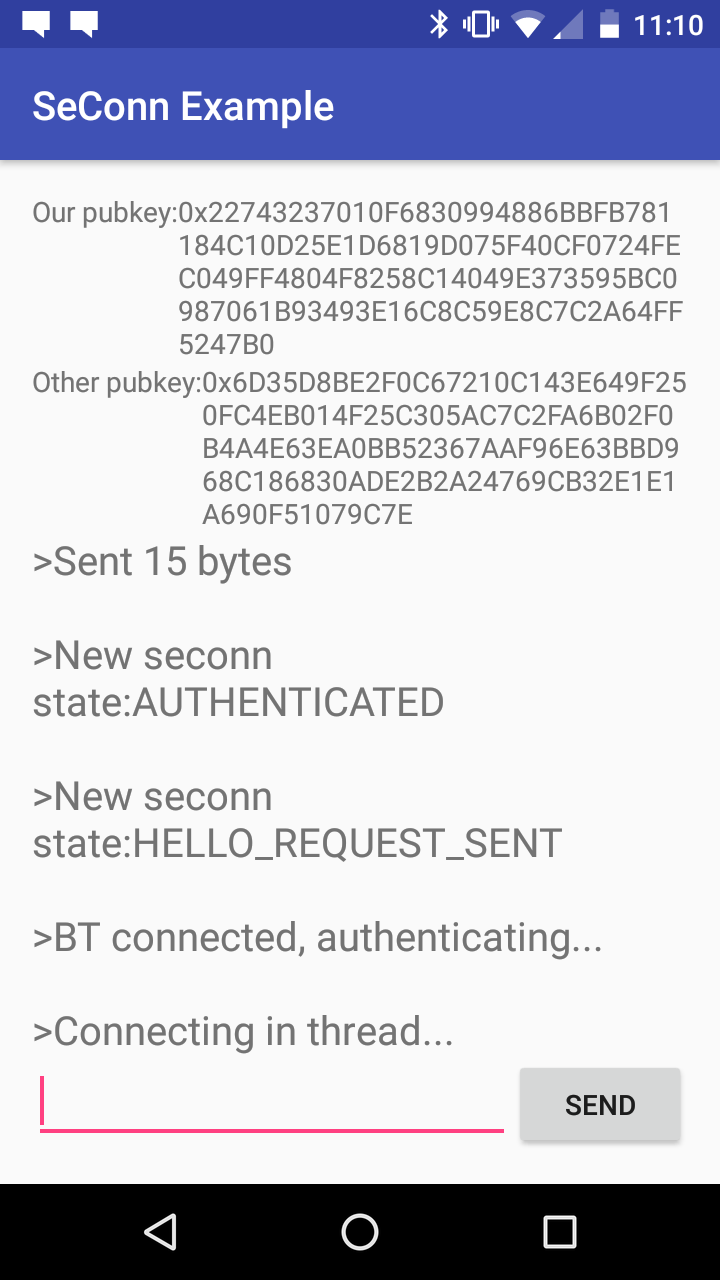
\includegraphics[height=0.6\textheight]{images/android.png}
\caption{Zrzut ekranu z przykładowej aplikacji implementującej protokół na platformę Android}
\label{fig:android}
\end{figure}

Przykładowa aplikacja mobilna skutecznie połączyła się z~urządzeniem AVR, a~przesyłane dane były prawidłowo deszyfrowane, co potwierdza że~implementacja algorytmów z~zewnętrzych bibliotek AVR oraz~implementacje wykonane w~ramach pracy są zgodne z~referencyjnymi implementacjami dostępnymi w~bibliotece standardowej języka Java na~platformie Android. Zrzut ekranu z~aplikacji przedstawiono na~rysunku \ref{fig:android}.


\chapter*{Podsumowanie}
\addcontentsline{toc}{chapter}{Podsumowanie}
\label{cha:podsumowanie}

Rodzina mikroprocesorów AVR jest często używana do~prototypowania urządzeń, które~przesyłają poufne dane lub~odbierają zdalne komendy, takich jak~bezprzewodowe tokeny, sensory oraz~inteligentne domy. Takie urządzenia powinny być zabezpieczone zarówno przed podsłuchiwaniem informacji jak~i~przed wykonywaniem nieupoważnionych poleceń.

W~pracy przedstawiono rozwiązanie w~postaci protokołu komunikacji oraz~biblioteki programistycznej dla urządzeń AVR, które~ma na~celu zapewnienie poufności, autentyczności oraz~integralności przesyłanych danych. Szczególny nacisk postawiono na~łatwość integracji.

Zaprezentowano różne metody uwierzytelniania i~wybrano algorytmy ECDH \emph{(ang. Elliptic Curve Diffie--Hellman)} oraz~AES użyty w~trybie ECBC-MAC \emph{(ang. Encrypt-last-block Cipher Block Chaining - Message Authentication Code)}. Za~ich przewagę nad~innymi rozwiązaniami uznano wydajność, niskie wymagania dotyczące pamięci operacyjnej oraz~jakość implementacji dostępnych na~urządzenia AVR. Dodatkowo w~celu zapewnienia poufności danych wybrano szyfrowanie algorytmem AES użytym w~trybie CBC. Ograniczeniem tej metody jest brak utajnienia przekazywania \emph{(ang. forward secrecy)}, a~więc ujawnienie klucza prywatnego dowolnego węzła pozwala na~odszyfrowanie całej przeszłej komunikacji.

Wykorzystano implementacje algorytmów ECDH oraz~AES z~bibliotek \emph{micro-ecc} oraz~\emph{AVR-Crypto-Lib}. W~ramach pracy stworzono implementacje trybów CBC, ECBC-MAC oraz~dopełniania PKCS\#7. Opracowano także protokół służący wymianie kluczy i~ustrukturyzowaniu przesyłanych danych.

Poprawność implementacji poszczególnych algorytmów zweryfikowano poprzez~porównanie zestawów danych wejściowych i~wyjściowych z~niezależnymi implementacjami w~aplikacjach internetowych oraz~w~języku Java na~platformie Android. W~celu potwierdzenia kompletności interfejsu programistycznego biblioteki stworzono przykładowe oprogramowanie na~platformę Arduino, które~oczekuje na~połączenie Bluetooth i~przekazuje uwierzytelnione dane na~połączenie szeregowe. Dodatkowo opracowano implementację protokołu w~języku Java oraz~przykładowe oprogramowanie na~platformę Android, które~nawiązuje połączenie Bluetooth i~pozwala na~szyfrowanie, uwierzytelnianie i~przekazywanie do~drugiego węzła wiadomości. Potwierdzono, że~komunikacja między implementacjami protokołu na~urządzenia AVR oraz~dla języka Java jest prawidłowa.

Przed wdrożeniem rozwiązania powinnien zostać przeprowadzony pełen audyt bezpieczeństwa zarówno protokołu jak~i~jego implementacji. Prawidłowy audyt powinien zostać przeprowadzony przez niezależny zespół, który~nie był powiązany z~projektem protokołu oraz~stworzeniem biblioteki, więc wykracza on poza zakres tej pracy.


% \listoffigures
\printbibliography[heading=bibintoc]

% itd.
\begin{appendices}
\chapter{Przykładowe wiadomości protokołu komunikacji}
\label{app:samplerecords}

\begin{table}[ht]
\centering
\caption{Budowa wiadomości typu HelloRequest}
\begin{BVerbatim}
# Nagłówek:
0x00 0x01 # wersja protokołu
0x00      # typ wiadomości: HelloRequest
0x00 0x40 # długość zawartości: 64 bajty

# Zawartość:
# 32 bajty współrzędnej X klucza publicznego
0x1F 0x92 0xDE 0xFF 0x6B 0xEE 0xFC 0x4D
0x51 0x2A 0x62 0xF4 0x60 0x1D 0x36 0x73
0x6F 0xEB 0x3F 0x1F 0x56 0x90 0xFD 0x85
0xB0 0x3C 0x56 0xD0 0xC0 0x52 0x6E 0x9B

# 32 bajty współrzędnej Y klucza publicznego
0xE8 0x60 0x84 0xB4 0xDE 0x73 0x65 0xB2
0x48 0xA6 0x15 0x79 0x7C 0xD9 0x4C 0xB6
0x56 0xE6 0xFA 0x3C 0x2F 0x3C 0x1C 0x8F
0xB2 0xE6 0x25 0xF8 0x66 0x2A 0x00 0xE4
\end{BVerbatim}
\label{fig:hellorequestsample}
\end{table}

\begin{table}
\centering
\caption{Budowa wiadomości typu HelloResponse}
\begin{BVerbatim}
# Nagłówek:
0x00 0x01 # wersja protokołu
0x01      # typ wiadomości: HelloResponse
0x00 0x60 # długość zawartości: 96 bajtów

# Zawartość:
# 16 bajtów kodu uwierzytelniającego
0x99 0x7B 0x57 0x10 0x7F 0x9C 0x1E 0xB3
0x1C 0x92 0x1B 0xFC 0x99 0x0C 0xCF 0x7D

# Zaszyfrowany klucz publiczny (64 bajty)
# z~uwzględnieniem dopełnienia PKCS#7 (16 bajtów)
0xF2 0x8A 0x7B 0xD4 0x04 0x80 0xAE 0xDC
0x7A 0x1D 0x04 0xEE 0x98 0x6D 0x9F 0xC5
0x22 0x4B 0x92 0x48 0x3E 0x65 0x79 0xC7
0xCB 0xCA 0xA9 0xC0 0xA1 0x7D 0x35 0x1F
0xFD 0x6F 0xE4 0x9E 0x62 0xBE 0x3F 0x1E
0xAC 0x32 0x03 0xF5 0x50 0x15 0xBE 0x0F
0x84 0xB9 0xF4 0xB6 0xF7 0x36 0x1D 0x3E
0x2D 0xD5 0xE3 0x10 0xBE 0xC4 0x39 0xC7
0x98 0x86 0x65 0x46 0x65 0xA9 0x5D 0xDE
0x4C 0x9D 0x03 0x00 0x55 0xE9 0xAF 0xC2
\end{BVerbatim}
\label{fig:helloresponsesample}
\end{table}

\begin{table}
\centering
\caption{Budowa wiadomości typu EncryptedData}
\begin{BVerbatim}
# Nagłówek:
0x00 0x01 # wersja protokołu
0x02      # typ wiadomości: EncryptedData
0x00 0x30 # długość zawartości: 48 bajtów

# Zawartość:
# 16 bajtów kodu uwierzytelniającego
0x6B 0xE7 0xBD 0xB6 0x23 0x98 0x1A 0x35
0xFF 0xBE 0xBB 0x38 0x3F 0xB1 0xF9 0x56

# Zaszyfrowane dane (dopełnione do~pełnego bloku AES)
0xD2 0x53 0xFF 0x58 0x99 0x94 0x36 0x24
0x1D 0x6B 0x4D 0x41 0x45 0xEF 0xD3 0x91
0x26 0x09 0xAB 0x91 0xC0 0x27 0x7C 0xAC
0x8E 0xFA 0xDA 0x24 0x9F 0xC6 0x22 0xBD
\end{BVerbatim}
\label{fig:encrypteddatasample}
\end{table}

\chapter{Przykładowe bloki kodu biblioteki}
\label{app:codesamples}

\definecolor{mygreen}{rgb}{0,0.6,0}
\definecolor{mygray}{rgb}{0.5,0.5,0.5}
\definecolor{mymauve}{rgb}{0.58,0,0.82}

\lstset{%
  basicstyle=\footnotesize\ttfamily,%
  keywordstyle=\bfseries\color{green!40!black},%
  commentstyle=\itshape\color{purple!40!black},%
  identifierstyle=\color{blue},%
  stringstyle=\color{orange},%
  breakatwhitespace=false,         % sets if automatic breaks should only happen at whitespace
  breaklines=true,                 % sets automatic line breaking
  captionpos=t,                    % sets the caption-position to bottom
  frame=single,	                   % adds a frame around the code
  keepspaces=true,                 % keeps spaces in text, useful for keeping indentation of code (possibly needs columns=flexible)
  language=C,                 % the language of the code
  rulecolor=\color{black}         % if not set, the frame-color may be changed on line-breaks within not-black text (e.g. comments (green here))
}


\begin{figure}[h]
\begin{lstlisting}[caption={Szyfrowanie CBC wraz z obsługą dopełnienia PKCS\#7},label={lst:encrypt}]
size_t _seconn_crypto_encrypt(void *destination, void *source, size_t length, aes128_key_t enc_key) {
    uint8_t *dest = (uint8_t*)destination;
    uint8_t *src = (uint8_t*)source;

    rng(dest, 16); // losowy wektor inicjalizacyjny
    memset(&ctx, 0, sizeof(aes128_ctx_t));

    aes128_init(enc_key, &ctx);

    aes128_enc(dest, &ctx);

    size_t i = 0;
    for(; i+16 <= length; i += 16) {
        memcpy(dest+16+i, src+i, 16);
        _seconn_crypto_xor_block(dest+16+i, dest+i);
        aes128_enc(dest+16+i, &ctx);
    }

    size_t pad_length = 16 - (length % 16);
    memset(dest+16+i, pad_length, 16);
    memcpy(dest+16+i, src+i, length - i);
    _seconn_crypto_xor_block(dest+16+i, dest+i);
    aes128_enc(dest+16+i, &ctx);

    return i+32;
}
\end{lstlisting}
\end{figure}

\begin{figure}
\begin{lstlisting}[caption={Odszyfrowanie CBC wraz z obsługą dopełnienia PKCS\#7},label={lst:decrypt}]
size_t _seconn_crypto_decrypt(void *destination, void *source, size_t length, aes128_key_t enc_key) {
    uint8_t *src = ((uint8_t*)source);
    uint8_t *dest = (uint8_t*)destination;

    memset(&ctx, 0, sizeof(aes128_ctx_t));
    aes128_init(enc_key, &ctx);

    size_t i = 0;
    for(; i+16 < length; i += 16) {
        memcpy(dest+i, src+i+16, 16);
        aes128_dec(dest+i, &ctx);
        _seconn_crypto_xor_block(dest+i, src+i);
    }

    size_t pad_length = dest[i-1];
    for(size_t j = 2; j <= pad_length; j++) {
        if (dest[i-j] != pad_length) {
            return 0;
        }
    }

    return i-pad_length;
}
\end{lstlisting}
\end{figure}

\begin{figure}
\begin{lstlisting}[caption={Obliczanie \gls{mac} dla wiadomości},label={lst:mac}]
void _seconn_crypto_calculate_mac(uint8_t *mac, void *message,
size_t length, aes128_key_t mac_key, aes128_key_t enc_key) {
    memset(&ctx, 0, sizeof(aes128_ctx_t));
    aes128_init(mac_key, &ctx);

    uint8_t *block = mac;

    memset(block, 0, 16); // wektor inicjalizacyjny wypełniony zerami

    // obliczenie ostatniego bloku szyfrowania w trybie CBC
    size_t i = 0;
    for(; i+16 <= length; i += 16) {
        _seconn_crypto_xor_block(block, ((uint8_t*)message)+i);
        aes128_enc(block, &ctx);
    }

    // szyfrowanie ostatniego bloku osobnym kluczem
    memset(&ctx, 0, sizeof(aes128_ctx_t));
    aes128_init(enc_key, &ctx);
    aes128_enc(block, &ctx);
}
\end{lstlisting}
\end{figure}

\chapter{Uzyskiwanie liczb losowych}
\label{app:randgen}

\definecolor{mygreen}{rgb}{0,0.6,0}
\definecolor{mygray}{rgb}{0.5,0.5,0.5}
\definecolor{mymauve}{rgb}{0.58,0,0.82}

\lstset{%
  basicstyle=\footnotesize\ttfamily,%
  keywordstyle=\bfseries\color{green!40!black},%
  commentstyle=\itshape\color{purple!40!black},%
  identifierstyle=\color{blue},%
  stringstyle=\color{orange},%
  breakatwhitespace=false,         % sets if automatic breaks should only happen at whitespace
  breaklines=true,                 % sets automatic line breaking
  captionpos=t,                    % sets the caption-position to bottom
  frame=single,	                   % adds a frame around the code
  keepspaces=true,                 % keeps spaces in text, useful for keeping indentation of code (possibly needs columns=flexible)
  language=C,                 % the language of the code
  rulecolor=\color{black}         % if not set, the frame-color may be changed on line-breaks within not-black text (e.g. comments (green here))
}

Biblioteka zaimplementowana w ramach pracy nie posiada żadnego źródła liczb losowych, mimo że jest ono potrzebne do jej prawidłowego funkcjonowania. Użycie biblioteki wymaga więc dostarczenia źródła liczb losowych przez osobę używającą biblioteki.

Najbezpieczniejszą metodą jest użycie dedykowanego, zewnętrznego generatora liczb losowych, lecz możliwe jest też wykorzystanie modułów dostępnych standardowo w mikropocesorach AVR. W bibliotece micro-ecc proponowana jest metoda wykorzystująca szum na niepodłączonym przetworniku analogowo-cyfrowym. Jej implementacja zaprezentowana jest w tabeli \ref{lst:rand}.

\begin{table}[!htb]
\caption{Generowanie liczb losowych w oparciu o wbudowany przetwornik analogowo-cyfrowy. Źródło: biblioteka micro-ecc}
\label{lst:rand}
\begin{lstlisting}
static int RNG(uint8_t *dest, unsigned size) {
  // Use the least-significant bits from the ADC for an unconnected pin (or connected to a source of 
  // random noise). This can take a long time to generate random data if the result of analogRead(0) 
  // doesn't change very frequently.
  while (size) {
    uint8_t val = 0;
    for (unsigned i = 0; i < 8; ++i) {
      int init = analogRead(0);
      int count = 0;
      while (analogRead(0) == init) {
        ++count;
      }
      
      if (count == 0) {
         val = (val << 1) | (init & 0x01);
      } else {
         val = (val << 1) | (count & 0x01);
      }
    }
    *dest = val;
    ++dest;
    --size;
  }
  return 1;
}
\end{lstlisting}
\end{table}

\chapter{Przepływ danych w przykładowym \mbox{oprogramowaniu}}
\label{app:samplediagram}

\begin{figure}[h]
\centering
\includegraphics[width=\textwidth]{images/sample-diagram.png}
\caption{Przepływ danych między komponentami w przykładowym \mbox{oprogramowaniu}}
\label{fig:samplediagram}
\end{figure}

\end{appendices}
% itd.


\end{document}
